% Chapter 1
\chapter{Typological overview} % Main chapter title
%\epigraph{The author bows before the reader, as well as the speakers involved in making this grammar, and the people that stand behind them. May you see the work that lies here, and know it. \textit{koin!}}{}
% i xatiike bwadut nyako i xafine, ma li xafavamale ale evaaya ko i tii-aen, ma li apuli caile. Ma gavwe xaleke i vaaya-ca, ka caihnan.

This chapter gives some introductory information on the typological profile of Vamale. %, as well as outlining the structure of the book.
Vamale, or Hmwaeke, is spoken on the northeast coast of New Caledonia, about half-way between the administrative centres of Hienghène and Touho. As a result of colonization, the language has gone from perhaps 2000 to 180 speakers, with most children speaking French instead. The geographical and historical context is described in \chapref{ChapterContext}. Vamale is a Southern Oceanic language, an eastern Voh-Koné variety in the Northern branch of Mainland New Caledonian.

Vamale ([ˈva.ma.le]) is an Oceanic language and conforms in many aspects to the canonical family profile established by \textcite{ross_morphosyntactic_2004}. It is head-first, uses verbs to express meanings for which European languages use other word classes, e.g. numerals and adjectives, and makes ample use of complex verb constructions. Vamale features dual and plural, as well as inclusive and exclusive pronouns. There is no gender, but animacy plays a role in object marking on verbs, among other things. It has no tense in the strict sense and uses aspectual and modal particles to express its predicate's temporal makeup. 

The language fits in neatly with its immediate, New Caledonian neighbors: like other Northern branch languages, Vamale has a large consonant inventory (35 phonemes), and features contrastive length and nasalization in vowels (20 phonemes). %The allophones of /o/ and /e/ were not yet described in detail for other languages in the area, though their distribution may well be a widespread phenomenon. 
Stress is mostly penultimate, with some influence of syllable weight, syllable position in the word, and (g-)wordhood status. %The phonology of the language also features a class of \textit{fortis} onsets, i.e. aspirated plosives, voiceless nasals and liquids, but also /h/, which attract stress and tend to nasalize the following vowel. 

However, there are also rarer facets to Vamale. Verb agreement, for example, shows tripartite alignment.
%``Active verbs" mark \gl{a} identically to \gl{S\textsubscript{A}}, and distinguish \gl{p}. This is an nominative-accusative alignment. However, another group of verbs, ``stative verbs", are intransitive, and mark the subject similarly to undergoers in transitive verbs, but are distinct from them. The distinction between \gl{S\textsubscript{P}} and \gl{p} is blurry, and may in time disappear. 
%This means that additionally to split-transitivity, which is common in the area, Vamale features a split along \gl{a}, \gl{S\textsubscript{A}} / \gl{S\textsubscript{P}} / \gl{p}. Some constructions, however, show yet different patterns: de-verbal nominalizations show ergative alignment for inanimate subjects and undergoers (\Cref{kan}). % the subject marker \textit{ka} is available to undergoers and is only obligatory for transitive subjects. The argument marked with \textit{ka-n} \qu{\gl{abs}-\gl{nspec}} is either an undergoer or an intransitive subject. The animacy of the participants plays a role in the obligatoriness of \textit{ka-n}, as it does in many aspects relating to nouns.  %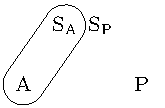
\includegraphics[\width=\linewidth]{figures/alignment}


\section{Phonology}
Vamale’s consonant and vowel phonemes are shown in Table \ref{tab:intro_cons} and Figure \ref{fig:intro_vowel}. As is typical of the area, there are many consonants, including labiovelarized and aspirate ones. Voiced plosives are pre-nasalized, and historical geminates have become ``fortis" consonants, either voiceless or aspirated plosives, or voiceless nasals and liquids. They attract stress and tend to nasalize the following vowel: [kʰɛ̃kʰɛ̃] \qu{parrot}, /han/ [hãn] \qu{to go}. 

%\begin{table}
%	\caption{Consonants in Vamale. Non-phonemes are in brackets.}
%	\begin{tabular}{p{1cm}lp{1.4cm}lp{1.2cm}lllp{1.2cm}l}
%		\lsptoprule
%		& Bilabial & Lab. Bilabial & Labiod. & Lab. Labiod. & Alv. & Palatal & Velar & Lab. Velar & Glott. \\
%		\midrule
%		Plosive & pʰ p ᵐb & (pʰʷ) pʷ ᵐbʷ &  &  & tʰ t ⁿd & (cʰ) c ⁿɟ & kʰ k ᵑɡ &  &  \\
%		Nasal & m̥ m & m̥ʷ mʷ &  &  & n̥ n & ɲ̊ ɲ & (ŋ̊) ŋ &  &  \\
%		Tap%or Flap
%		&  &  &  &  & (ɾ) &  &  &  &  \\
%		Fricative &  &  & f v & fʷ vʷ & s &  & x ɣ & xʷ & h \\
%		Approx. &  &  &  &  &  & j &  & w &  \\
%		Lat. Approx. &  &  &  &  & l l̥ &&&&\\
%		\lspbottomrule
%	\end{tabular}

%\end{table}

\begin{table}
\caption{Consonants in Vamale. Non-phonemes are in brackets.}
\begin{tabular}{llllllllll}
\lsptoprule
                   & Bilabial & Lab. Bilab. & Labiod. & Lab. Labiod. \\\midrule
Plosive            & pʰ p ᵐb & (pʰʷ) pʷ ᵐbʷ &           &              \\
Nasal              & m̥ m     & m̥ʷ mʷ        &           &            \\
Tap                &         &              &           &              \\
Fricative          &         &              & f v       & fʷ vʷ        \\
Approximant        &         &              &           &              \\
Lat. Approx.       &         &              &           &              \\\midrule
                   & Alveolar & Palatal & Velar & Lab. Velar & Glott. \\\midrule
Plosive            & tʰ t ⁿd & (cʰ) c ⁿɟ & kʰ k ᵑɡ &    &  \\
Nasal              & n̥ n     & ɲ̊ ɲ       & (ŋ̊) ŋ   &    &  \\
Tap                & (ɾ)     &           &         &    &  \\ % or flap
Fricative          & s       &           & x ɣ     & xʷ & h \\
Approximant        &         & j         &         & w  &  \\
Lat. Approx.       & l l̥     &           &         &    &\\
\lspbottomrule
\end{tabular}
\label{tab:intro_cons}
\end{table}

\begin{figure}
	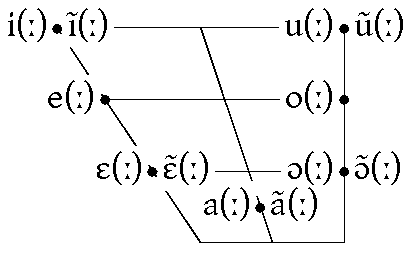
\includegraphics[width=0.4\linewidth]{figures/vowel}
	\caption{Vowel qualities in Vamale}
	\label{fig:intro_vowel}
\end{figure}


There are five phonemic vowel qualities /a, e, i, o, u/, with phonemic nasality and length: \textit{tha} \qu{assertive particle} \textit{thâ} \qu{excrement} \textit{the} \qu{algae} \textit{thê} \qu{rock} \textit{tho} \qu{call} \textit{thu} \qu{banyan tree}. The phonemic status of [ɔ̃] and [ũ] is a matter of analysis, as there are no minimal pairs with oral counterparts.

All vowels following nasal stops tend to be nasalized. There is limited allophonic variation in vowels, concerning chiefly /a/ pronounced [ɑ] after labiovelar approximants and /u/, which is pronounced [ʏ] after /i/, e.g. \textit{vwa} \qu{do} [vʷɑ], \textit{si-ung} \qu{hand-1\gl{sg}.\gl{poss}} [sʏŋ]. Possibly as a result of contact with neighbouring languages featuring more vowel phonemes, /o/ and /e/ have more open allophones in short closed syllables ([sɛn] \qu{poison}) or before a consonant in the same syllable ([ɔːt] \qu{rope, tendon, vine}), than in open ones ([ko] \qu{at}) or in long nasal-bounded ones ([soːm] \qu{swim}). Consonants may be lenited or fricativized in fast speech, and phonemically voiceless nasals and liquids may not be audibly realized as such (e.g. [m̥ũ̠ːn] $\sim$ [mũːn] \qu{smoke, dust}), but this is not a regular process.

Syllables never feature two consonants one after the other ((C)V(:)(C)), and may only end on a vowel, a nasal, or /p,t,c,k/, e.g. [tʰu] \qu{banyan tree}, [tʰuːp] \qu{bathe}, [tuːn] \qu{clan}. The early French loanword \textit{cheval} [ʃø.val] \qu{horse} was phonologically adapted to [so.van], as -l cannot occur syllable-finally.

Whether Vamale has true dipthongs (where both vowels occur in the same syllable) depends on the analysis. The second vowel in a syllable is always either /i/ or /u/ and not functionally distinct from the glides /j/ and /w/. Either Vamale has only dipthongs ending on /i/ or /u/, or Vamale has no diphthongs but may end the syllable on a glide. 

\begin{sloppypar}
The main stress is on the second-to-last (penultimate) syllable for most words, or on the first of three syllables, e.g. [ˈvʷaⁿ.di] \qu{peel by hand}, [ˈa.pu.li] \qu{person}. Vamale does not have native phonological words with more than three syllables: though morphologically speaking, there are longer structures, speakers split these up into intonational units of three syllables maximum, e.g. \textit{xa-vwa-tau} \qu{\gl{nmlz}-do-impact (fisherman)} is pronounced [ɣa.vʷa.ˈtau] but the four-syllable word \textit{xa-vwa-buke} \qu{\gl{nmlz}-do-flower (flower seller)} is pronounced [ˌɣa.vʷa.ˈᵐbu.ke].
Derivational prefixes, transitivity marking suffixes, possessive markers and other grammatical morphemes may behave differently stress-wise: bisyllabic morphemes may be counted as one stress unit, and some suffixes are even ignored completely, e.g.
\end{sloppypar}

\begin{itemize}
\item {[}ˈmu.lip] \qu{life}
\item {[}mu.ˈlip.ga.vwe] \qu{life-2\gl{pl}.\gl{poss}}
\item {[}ˈɲ̊i.mã] \qu{heart, thought}
\item {[}ˈɲ̊i.mã.ke] \qu{to think}
\end{itemize}

\section{Example sentences}

The example sentences have three different sources. The reference is given in brackets under the examples. Most of the examples were elicited or found in recorded free text (see \sectref{sec:Meth} for details on recording and transcription methods) and can be traced to an audio file via the FLEx database uploaded to ELAR. The text collection on FLEx can be ordered by ``Abbreviation". The abbreviations used correspond to the code of one or two letters and sometimes a number, and the number after the colon is the line in the text (e.g. AG1:394). Other examples were not audio-recorded, but noted in writing. Their references start by the date of the entry (e.g. 180722 p.93, or 07.11.18 p.93). Other examples were transcribed from audio files but not yet included in a Flex file, and are referenced by the filename and the time stamp, also on ELAR (e.g. vamale-181107.jpnelemwa-04: 00:00:30- 00:00:32). Unreferenced examples were constructed for the purpose of writing up the grammar, and checked with speakers. 

\section{Person forms and demonstratives} 

Vamale distinguishes subject (\gl{a}\slash\gl{S\textsubscript{A}}) and object (\gl{p}) person forms (\Cref{tab:intro_markers}). There are three numbers, singular, dual, and plural. The language distinguishes inclusive (\qu{us and you}) and exclusive (\qu{us but not you}) first person forms. Object pronouns are never independent as seen in (\ref{ex:intro_obj}), whereas the others may be attached to the verb or occur in a free form (\ref{ex:intro_both}). 

\begin{table} 
	\caption{Subject and object markers for active and stative verbs}
	\begin{tabular}{lllll}
		\lsptoprule
		& & cross-indexes & \multicolumn{2}{c}{pro-indexes}  \\\cmidrule(lr){3-3}\cmidrule(lr){4-5}
		&	Free form	& \gl{a}=/ \textsc{s\textsubscript{a}}= & -\textsc{s\textsubscript{p}} & -\gl{p}\\
		\midrule
		1\gl{sg} & \textit{io} & \textit{e=} & \textit{-o(ng)} & \textit{-o} \\
		1\gl{du}.\gl{incl}& \textit{gasu} & \textit{gasu=} & \textit{-gasu} & \textit{-kaeu}\\
		1\gl{pl}.\gl{incl} & \textit{gaa/gase} &\textit{ga(se)=}&\textit{-gaa}&\textit{-kaa}\\
		1\gl{du}.\gl{excl} & \textit{abu} & \textit{abu=} & \textit{-abu} & \textit{-(a)bu}\\
		1\gl{pl}.\gl{excl} & \textit{abe}& \textit{abe=} & \textit{-abe} & \textit{-(a)be}\\
		2\gl{sg} & \textit{go} &\textit{go=} & \textit{-go} & \textit{-ko}\\
		2\gl{du} & \textit{gau} & \textit{gau=} & \textit{-gau} & \textit{-kau}\\
		2\gl{pl} &\textit{gavwe}& \textit{gavwe=} & \textit{-gavwe} & \textit{-kavwe}\\
		3\gl{sg} & \textit{ia} & \textit{a=} & \textit{-(e)a} & \textit{-(e)a}\\
		3\gl{du} & \textit{lu} &\textit{lu=} & \textit{-lu} & \textit{-lu}\\
		3\gl{pl} & \textit{le} & \textit{le=} & \textit{-le} & \textit{-le}\\
		\lspbottomrule
	\end{tabular}
	\label{tab:intro_markers}
\end{table}

\ea[]{\label{ex:intro_both}
\gll e=xale-ko ka=yo\\
 1\gl{sg}=see-2\gl{sg}.\gl{obj} \gl{sbj}=1\gl{sg}\\
\glt \qu{I see you.}}
\z


\ea[*]{\label{ex:intro_obj}
\gll e=xale go \\
 1\gl{sg}=see 2\gl{sg}\\
\glt (for: \qu{I see you})}
\z

Most personal pronouns look similar to their free form counterpart, and were probably historically derived from them. Suffixes indexing objects and stative subjects (\gl{S\textsubscript{P}}) always refer to people or animals, whereas active subjects (\gl{a} and \gl{S\textsubscript{A}}) do not mark the animacy of their referent.

\ea
%\a
\gll phwaat i=thala\\
 clean \gl{def}.\gl{sg}=knife\\
\glt \qu{The knife is clean.}
\z

%\a
\ea
\gll a=tabo i=thala\\
 3\gl{sg}=sit \gl{def}.\gl{sg}=knife\\
\glt \qu{The knife lies (there).}
\z

The stative subject (\gl{S\textsubscript{P}}) and the object suffixes cannot co-occur with an independent person form (pro-indexing person forms).

Demonstratives distinguish number (singular, dual, plural) as well as proximity (proximal \textit{-hni}/distal (\textit{-na})). %Though they were probably transparently formed in the past, the current usage distinguishes the forms along more opaque lines: \textit{ena} is the only possible form useable to agree with a previous statement. 
The demonstratives resemble in part the articles, which are also listed in \Cref{tab:intro_demonstratives}. Two demonstratives, \textit{na} and its repeated form \textit{ha} (meaning it is used if the information is repeated, often with insistence), cannot be used as predicates, nor do they mark number or proximity: they are deictic pronouns that take a nominal predicate. They are illustrated in (\ref{ex:na}) and (\ref{ex:ha}).

\begin{table}
	\caption{Demonstrative pronouns and articles}
	\begin{tabular}{lll ll}
		\lsptoprule
		& \multicolumn{2}{c}{Demonstrative} & \\
		& \multicolumn{2}{c}{pronouns} &\multicolumn{2}{c}{Articles}\\\cmidrule(lr){2-3}\cmidrule(lr){4-5}
		& Proximal & Distal	&\gl{spec} and \gl{def}& \gl{spec} and \gl{indf}\\\midrule
		\gl{sg} & \textit{e-hni} & \textit{e-na}& \textit{i} & \textit{(e)ca}\\
		\gl{du} & \textit{muu-hni} & \textit{muu-na} & \textit{mu} & \textit{muca} \\
		\gl{pl} & \textit{ni-e-hni} & \textit{ni-e-na} & \textit{li} / \textit{ni} & \textit{ca(been)}\\	
		\lspbottomrule
	\end{tabular} 
	\label{tab:intro_demonstratives}
\end{table}

\ea
%\ea
\label{ex:na}
\gll na yo \\
 \gl{dem} 1\gl{sg}\\
\glt \qu{It's me.}
\z

\ea \label{ex:ha}
%a
\gll li=xa-vuki vai ko-n thexhwaade, {\ob}ha{\cb} {\ob}li=kalen{\cb}\\
\gl{def}.\gl{pl}=\gl{nmlz}-stem stone on-\gl{nspec} T. \gl{dem}.\gl{rep} \gl{def}.\gl{pl}=K\\
\glt \qu{The owners of Thexhwaade rock, are the Kalens (and no-one else).} {[DP:12]}
\z


\section{Element order}

Like many other Oceanic languages in the area, Vamale is predominantly VOS \REF{ex:vos}, though the pragmatically most important element (usually the subject) is frequently fronted \REF{ex:vos2}. Modifiers follow the modified, as in \REF{ex:vos1}.


\ea\label{ex:vos}
\gll le=fwii i=jamwa-m ka=li=mani\\
 3\gl{sg}=wake.up \gl{def}.\gl{sg}=father-1\gl{sg}.\gl{poss} \gl{sbj}=\gl{def}.\gl{pl}=bird\\
\glt \qu{The birds wake my father up.}
\z


\ea\label{ex:vos2}
\gll i=jamwa-m, go=fwi-a\\
 \gl{def}.\gl{sg}=father-2\gl{sg}.\gl{poss} 2\gl{sg}=wake.up-3\gl{sg}\\
\glt \qu{Your father, you wake him up.}
\z


\ea \label{ex:vos1}
\gll go=fwii i=jamwa-m a=meebam\\
 2\gl{sg}=wake.up \gl{def}.\gl{sg}=father-2\gl{sg}.\gl{poss} \gl{rel}=sleep\\
\glt \qu{You wake up your sleeping father.}
\z
\section{Argument coding}

Vamale has several strategies for argument coding. Its differences from those of Vamale's closest relatives, are likely due to contact with surrounding languages. (Pro)nominal subjects are marked differently from objects. As with all Northern New Caledonian languages, subject noun phrases of all verb classes are marked with dedicated (pro-clitic) particle, in this case \textit{ka}, e.g. (\ref{ex:active}), or \textit{a} when following a consonant-final word (e.g. \textit{a=soom a=ya} \qu{she=swims \gl{sbj}=she}). However, \textit{ka} \qu{\gl{sbj}} is optional and unusual for intransitive subjects, while it is obligatory for transitive ones. This is a tripartite alignment system as illustrated in \Cref{fig:intro_alignment1}, and found in other Voh-Koné languages as well. 

\begin{figure}
% % % 	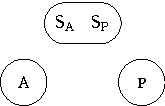
\includegraphics[width=0.3\linewidth]{figures/noun_alignment}
	\begin{tikzpicture}
		\topleftnode[sa]{\gl{S\textsubscript{A}}}
		\toprightnode[sp]{\gl{S\textsubscript{P}}}
		\leftnode[a]{\gl{a}}
		\rightnode[p]{\gl{p}}
		\draw (a) circle (11.2pt);
		\draw (p) circle (11.2pt);
		\draw \convexpath{11.2pt}{sa,sp};
	\end{tikzpicture}
	\caption{Alignment of noun phrases}
	\label{fig:intro_alignment1}
\end{figure}

``Active verbs" may be either transitive or intransitive. They index transitive subjects \gl{a} identically to agent-like intransitive subjects \gl{S\textsubscript{A}}, and distinguish them from objects \gl{p}, as in (\ref{ex:active}). Another group of verbs, ``stative verbs", are always intransitive (\ref{ex:stative}), and mark the subject \gl{S\textsubscript{P}} similarly to undergoers in transitive verbs, but are distinct from them (see \Cref{tab:intro_markers} for the forms). %The distinction between \gl{S\textsubscript{P}} and \gl{p} forms is blurry depending on the speaker, and may in time disappear. The distinction is not found in western Voh-Koné where a strictly split-transitive system marks \gl{S\textsubscript{P}} like \gl{p} and like possessors as well, but instead the Vamale distinction mirrors the one found in Pije and Nemi spoken to the north of Vamale.
It is a tripartite system shown in \Cref{fig:intro_alignment2}, but differently so than the one for noun phrases.


	\ea
	%\ea
	\label{ex:active}
	\gll e=bune i=balô ka=yo\\
	 1\gl{sg}=steal \gl{def}.\gl{sg}=ball \gl{sbj}=1\gl{sg}\\
	\glt \qu{I steal the ball.}
	\z
	
	
%	\ea
	\ea\label{ex:stative}
	
	\gll xawe-ong ka=yo\\
	 young-1\gl{sg} \gl{sbj}=1\gl{sg}\\
	\glt \qu{I am young.}
		\z

	
\begin{figure}
\begin{floatrow}
\captionsetup{margin=.05\linewidth}
\ffigbox{%
% 	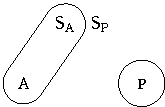
\includegraphics[width=0.3\linewidth]{figures/verb_alignment}
	\begin{tikzpicture}
		\topnode{}
		\topleftnode[sa]{\gl{S\textsubscript{A}}}
		\toprightnode[sp]{\gl{S\textsubscript{P}}}
		\leftnode[a]{\gl{a}}
		\rightnode[p]{\gl{p}}
		\draw \convexpath{11.2pt}{a,sa};
		\draw (p) circle (11.2pt);
	\end{tikzpicture}}
	{\caption{Alignment with verbs}
	\label{fig:intro_alignment2}}

% % 	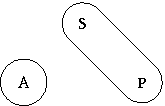
\includegraphics[width=0.3\linewidth]{figures/kan_alignment}
\ffigbox{%
	\begin{tikzpicture}
		\topnode[s]{\gl{s}}
		\leftnode[a]{\gl{a}}
		\rightnode[p]{\gl{p}}
		\draw \convexpath{11.2pt}{p,s};
		\draw (a) circle (11.2pt);
	\end{tikzpicture}}
	{\caption{Alignment with \textit{ka-n} nominalizations}
	\label{fig:intro_alignment3}}
\end{floatrow}
\end{figure}

This means that additionally to split-transitivity, which is common in the area, Vamale features a split along \gl{a}, \gl{S\textsubscript{A}}\slash\gl{S\textsubscript{P}}\slash\gl{p}. Some constructions, however, show yet different patterns: de-verbal nominalizations exhibit ergative alignment for inanimate subjects and undergoers, see (\ref{ex:intro_erg}) and \Cref{fig:intro_alignment3}. This last strategy is most likely related to possessive constructions, and uses similar morphemes (\textit{ka} and \textit{ka(-n)}, respectively). %It may have been calqued from a similar Cèmuhî construction, Vamale's neighbour to the south.
With active verb subjects (S/A-arguments), the cross-indexes occur under all circumstances, but with patient objects (P-arguments) and stative subjects, the pro-indexing suffixes cannot co-occur with the full nominal. 

\ea \label{ex:intro_erg}
\gll i=hun-coopwi ka i=vai\\
 \gl{def}.\gl{sg}=\gl{nmlz}-bury \gl{link} \gl{def}.\gl{sg}=stone\\
\glt \qu{the burying of the stone}
\z


\ea
\gll i=ape-tabo ka i=vai\\
 \gl{def}.\gl{sg}=\gl{nmlz}-sit \gl{link} \gl{def}.\gl{sg}=stone\\
\glt \qu{the position of the stone}
\z

\begin{sloppypar}
Ditransitive constructions distinguish human recipients from non-human ones; \textit{nya-si-} \qu{put-hand} is used for humans and \textit{nya-ko} for non-humans and humans in informal contexts alike. The markers can be discontinuous, as seen in \REF{ex:intro_nyasi_gift}. The constituent order is relatively free and subject to pragmatic preferences (compare (\ref{ex:intro_nyasi_demand}) and (\ref{ex:intro_nyasi_gift})).
\end{sloppypar}


\ea\label{ex:intro_nyasi_demand}
% \langinfo{}{}{} 
\gll e=ila-ke nyasi-m i=vai ka=yo\\
 1\gl{sg}=make.request-\gl{tr} \gl{ben}-2\gl{sg}.\gl{poss} \gl{def}.\gl{sg}=stone \gl{sbj}=1\gl{sg}\\
\glt \qu{I (politely) ask you for the stone (lit. I request the stone from you).}
\z


\ea\label{ex:intro_nyasi_gift}
% \langinfo{}{}{} 
\gll a=nya li=saleka-n si li=apuli\\
 3\gl{sg}=give \gl{def}.\gl{pl}=property-3\gl{sg}.\gl{poss} \gl{ben} \gl{def}.\gl{pl}=person\\
\glt \qu{He gives his things away to the people.} 
\z

\section{Word classes}

 Verbs can be sub-classified into free and dependent verbs, stative (i.e. state-like) and active (activity-like) ones. Nouns distinguish classifiers and different sub-classes nouns depending on their possessive morphology and ability to head a phrase. There are a number of subordinators, tense/aspect/mood markers, different kinds of pronouns etc. Typologically interesting aspects include the lack of a dedicated numeral class, whose function is instead covered by stative verbs, e.g. \textit{thaloo-lu} \qu{two-3\gl{du}} \qu{there are two, they are two}. There are no adjectives either, as is common in the area, where predicative adjectival functions are covered by stative verbs, and attributive ones by relative clauses, as seen in (\ref{ex:intro_pred}) and (\ref{ex:intro_att}).

\ea
\label{ex:intro_pred}
\gll vun-eo(ng)\\
 blue-1\gl{sg}\\
\glt \qu{I am blue.}
\z


\ea\label{ex:intro_att}
\gll a=thêên a i=thamo (a=) en maa-n\\
 3\gl{sg}=run \gl{sbj} \gl{def}.\gl{sg}=woman \gl{rel}= fine face-3\gl{sg}.\gl{poss}\\
\glt \qu{The beautiful (lit. `fine-faced') woman is running.}
\z

%\begin{table}
%	\centering
%	\caption{Main word classes}
%	\begin{tabular}{ll}
%		Main classes (that fill a unique slot) & Subclasses (based on morphosyntactic differences) \\
%		\midrule
%		\multirow{3}{*}{Nouns} & Alienable Nouns\\
%							& Inalienable Nouns\\
%							&Pronouns (personal, demonstrative) \\
%	
%		Articles &\\
%	
%			Subject proclitics		&\\		
%		TAM markers&\\
%		\multirow{3}{*}{Verbs}& Active Verbs\\
%			& Stative Verbs\\
%			& Manner Verbs\\
%		Adverbs&\\
%		Prepositions&\\
%			Subject marker \textit{ka}&\\
%		Conjunctions&\\
%		\multirow{3}{*}{Subordinators}&Complementizers\\
%		& Subordinators\\
%		& Relativizer\\
%		Negation markers&\\
%		Quantifiers&\\
%	\end{tabular}
%\label{tab:intro_wc}
%\end{table}

The negator \textit{cipa}, the assertive marker \textit{tha}, and epistemic mood markers such as the irrealis conditional \textit{cama} \qu{if ever} can precede both verbal and nominal (i.e. equational) clauses, see (\ref{ex:intro_clause}).

\ea \label{ex:intro_clause}
\gll tha cipa=le=hân\\
 \gl{ass} \gl{neg}=3\gl{pl}=go\\
\glt \qu{They did not leave.}
\z

\section{Verbs and verb phrases}

Verbs in Vamale are either free or dependent, meaning they may head a verb phrase or not. Serial verb constructions and other complex verbs are common and a productive way to express a series of related events, a complex action, or just to modify a verb.

Free verbs may take person-indexing proclitics (in the case of active verbs) or suffixes (for stative verbs), but usually omit them if in the imperative or prohibitive mood. The latter is marked by a particle \textit{cipii} (\ref{ex:intro_cipii}), related to the predicate negator \textit{cipa} (\ref{ex:intro_cipa}).



\ea\label{ex:intro_cipii}
\gll cipii (go)=see!\\
 \gl{proh} 2\gl{sg}=cry\\
\glt \qu{Don't (you) cry!}
\z

	
\ea\label{ex:intro_cipa}
\gll cipa=go=xaleke?\\
 \gl{neg}=2\gl{sg}=see\\
\glt \qu{Don't you see?}
\z


A set of particles precede the predicate to mark aspect and mood, as in \REF{ex:intro_bwa}. They can be combined, with sometimes idiosyncratic new meanings, and are sensitive to the verb's semantic nature (``aktionsart").
Their basic members are the imperfective \textit{bwa(n)}, perfective \textit{pa}, perfect \textit{ja}, progressive \textit{koon}, irrealis \textit{(b)o}, continuative\slash realis \textit{balan}, and frequentative\slash iterative \textit{mu}.

Verbs do not inflect for tense; indeed there are no dedicated tense markers, though the imperfective marker \textit{bwa} and the irrealis \textit{bo} are  used to suggest future actions (as in ex. \ref{ex:intro_bwa}), progressive \textit{koon} implies (relative) present tense and the perfectives \textit{pa} and \textit{ja} refer to the past. 

\ea \label{ex:intro_bwa}
\gll e=bwa=yahan\\
 1\gl{sg}=\gl{ipfv}=leave\\
\glt \qu{I will leave, I am just leaving.}
\z


\section{Derivation}

Many verbs are nominalized simply by putting an article before them, and some nouns can be verbalized by adding the transitive suffix \textit{-ke}. Indeed, entire verb phrases with arguments (but not tense or aspect markers) may be nominalized with an article. Other derivational affixes are the locative nominalizer \textit{ape-} (\textit{ape-tabo} \qu{place-sit; chair}), the manner nominalizer \textit{hun-} (\textit{hun-mata} \qu{manner-sing; singing style}), the instrumental \textit{e-} and the agentive \textit{xa-}. While \textit{e-} is ancient, others can be transparently reconstructed as former preposed nouns: \textit{ape-n} \qu{trace}, \textit{xa-} from \textit{xayu} \qu{man, male}. See (\ref{ex:intro_erg}) for two examples of nominalizers. 

\section{Nouns and noun phrases}

Nouns can be classified as inalienable (obligatory possessive morphology) or, if the morphology can be omitted, as alienable (see \Cref{tab:intro_PossSuffix1} for the suffixes). This follows a semantic logic, as is typical of Oceanic languages: inalienable nouns include kinship terms, body parts, and other parts of an individual (e.g. \textit{dedoo-ng} \qu{shadow-my}). Nouns can be possessed via direct (i.e. suffixal) or indirect (i.e. clitical) constructions, which usually depends on their alienability. However, a small number of nouns are alienable yet have directly possessed forms showing etymological stems: \textit{fedat} \qu{blood}, \textit{fedal-ong} \qu{my blood}. Nouns are either specific (using a definite or an indefinite article), or generic (without an article), as shown in (\ref{ex:intro_gen}). Number is also shown on the article instead of the noun. The only type of inflection found on nouns is adpossessive person marking (for animate possessors), and the formerly independent linker \textit{-n} indicating that the noun is possessed by a usually post-poned fully nominal possessor (\ref{ex:intro_poss}). Vamale has no adjectives; instead, nouns are modified via relative clauses. 


	\ea \label{ex:intro_gen}
	\gll i=xa-vwa i=xam\\
	 \gl{def}.\gl{sg}=\gl{nmlz}-do \gl{def}.\gl{sg}=mat\\
	\glt \qu{the maker of the mat}
	\z
	
	
	\ea
	\gll i=xa-vwa xam\\
	 \gl{def}.\gl{sg}=nmlz-do mat\\
	\glt \qu{the mat-maker, the maker of mats}
		\z


\begin{table}
	\caption{Possessive suffix paradigms}
	\begin{tabular}{llll}
		\lsptoprule
		&    & \multicolumn{1}{c}{inalienable} & \multicolumn{1}{c}{alienable}\\\midrule
\gl{sg} &	1&	\textit{-ng}&	\textit{-eong}\\
		&	2&	\textit{-m}&		\textit{-go}\\
		&	3&	\textit{-n}&		\textit{-ea}\\
		\midrule
\gl{du} &	1\gl{incl}&	\textit{-ju}&	\textit{-gaeu}\\
		&	1\gl{excl}&	\textit{-bu}&	\textit{-abu}\\
		&	2&	\textit{-u}&	\textit{-gau}\\
		&	3&	\textit{-lu}&		\textit{-lu}\\
		\midrule
\gl{pl} &	1\gl{incl}&	\textit{-je}&	\textit{-gaa}\\
		&	1\gl{excl}&	\textit{-be}&		\textit{-abe}\\
		&	2&	\textit{-vwe}&		\textit{-gavwe}\\
		&	3&	\textit{-le}&		\textit{-le}\\
		\lspbottomrule
	\end{tabular}
	\label{tab:intro_PossSuffix1}
\end{table}

\section{Possessive constructions and compounds}
An adpossessor nominal is unmarked (e.g. \textit{udee} in (\ref{ex:intro_poss})) and follows the possessed noun, which in turn carries a linker suffix \textit{-n} if the stem ends on a vowel, e.g. \textit{mwa-n}. 



	\ea\label{ex:intro_poss}
	\gll mwa-n udee\\	
	 house-\gl{link} medicine\\
	\glt \qu{pharmacy}
	\z
	
	\ea\label{ex:intro_poss2}
	\gll inya-m\\
	 mother-2\gl{sg}.\gl{poss}\\
	\glt \qu{your mother}
	\z

When the possessed noun is an inalienable term, it is marked for adpossessor person (see \Cref{tab:intro_PossSuffix1}, and (\ref{ex:intro_poss2})). Nominal compounds (\ref{ex:nom-comp}) are formally very similar to some nouns modified by relative clauses (\ref{ex:nom-rel}). However, the latter forbids articles in the modifying noun phrase, and the stress contours differ: a compound noun is treated as one unit instead of several. 


\ea\label{ex:nom-comp}
[iˌtʰamõˈxa.o.m̥ũ]\\
\gll i=thamo-xhaohmu\\
 \gl{def}.\gl{sg}=woman-elder\\
\glt \qu{the old woman}
\z


\ea\label{ex:nom-rel}
[iˈtʰaˌmõ ˈɣaˌsoːm]\\
\gll i=thamo (a= i=) xa-hnyimake\\
 \gl{def}.\gl{sg}=woman (\gl{rel}= \gl{def}.\gl{sg}=) \gl{nmlz}=swim\\
\glt \qu{the swimmer woman, the woman who swims}
\z

\section{Prepositions}

Vamale prepositions can be divided into prepositions proper (e.g. \textit{patemwano} \qu{very close by}) and ``relational nouns", which have nominal morphology and can sometimes be linked to a (voiced) nominal counterpart, see \Cref{tab:intro_prep}. 

\begin{table}
\caption{A selection of prepositions}
\begin{tabular}{l@{~}l  l@{~}l}
	\lsptoprule
	\multicolumn{2}{l}{Relational nouns}&\multicolumn{2}{l}{Related noun or meaning}\\
	\midrule
	\textit{cela-n}        & \qu{next to}                      & \textit{jela-n} & \qu{side}\\
	\textit{pwa-n}         & \qu{on top of}                    & \textit{bwa-n}  & \qu{head, top}\\
	\textit{can-hawâ-n}    & \qu{facing}                       & \multicolumn{2}{l}{in-face-\gl{link}}\\
	\textit{cake-bwa-n}    & \qu{on the other riverbank}       & \multicolumn{2}{l}{scoop.water-top-\gl{link}}\\
	\textit{cai-n}         & \qu{behind an animate entity}     & \textit{jèi-n} & \qu{back} (Cèmuhî)\\
	\textit{xala-n}        & \qu{under}                        & \\
	\textit{(can) dawee-n} & \qu{(in-) between}                & \\
	\textit{ca-n}          & \qu{in, at}                       & \\
	\textit{ko-n}          & \qu{on, at}                       & \\
	\textit{pathabua-n}    & \multicolumn{3}{@{}l}{\qu{before (spatial and temporal)}} \\
	\lspbottomrule         
\end{tabular}
\label{tab:intro_prep}
\end{table}

\begin{sloppypar}
Prepositions introduce adjuncts like points in time or locations, but also oblique noun phrases (\textit{nyako, nyasi}, see (\ref{ex:intro_nyako})), causes (\textit{ko}), adverbial clauses (\textit{can}), and subordinate clauses (\textit{ma, koma, cama}). %They are clitics, meaning they are syntactically own words, but do not carry stress. %yeah well there's ko,ma 'xaleke, 'canbwan, pwan 'jelan,jati etc
\end{sloppypar}

\ea \label{ex:intro_nyako}
\gll e=vi nyakoo-m\\
 1\gl{sg}=say \gl{obl}-2\gl{sg}.\gl{poss}\\
\glt \qu{I say (it) to you.}
\z

\section{Subordinate clauses}

There are relative clauses, adverbial clauses, conditional clauses, and, related to the latter, complement clauses. Relative clauses are the main way to modify a noun, adverbial clauses are one of the most important strategies to modify a verb, and many verbs require a complement clause. Relative clauses are introduced by the pro-clitic \textit{a}, probably related to the third person singular cross-indexing pronoun (\textit{a}), see (\ref{ex:intro_rel}). 

\ea \label{ex:intro_rel}
\gll li=dube a=xakoop(-le)\\
 \gl{def}.\gl{pl}=deer \gl{rel}=wild-3\gl{pl}\\
\glt \qu{the wild deer}
\z

Both the relativizer \textit{a} and the subject-indexing pro-clitic may be omitted (the latter only if the subject of the main clause is the same as the relative one). Subordinate clauses are formally identical to main clauses in both word order and content; only the subordinator marks the subordinate clause as such. Coordinate clauses are identical to subordinate ones except that that the subordinate clause may be fronted (\ref{ex:sub}), while coordinate clauses have a fixed order.

\ea \label{ex:sub}
\gll {\ob}ma le=tiike{\cb}, tha vwa ca=peipa la\\
 \gl{subr} 3\gl{pl}=write \gl{ass} \gl{exist} \gl{indf}.\gl{sg}=paper here\\
\glt \qu{For them to write, there is some paper here.}
\z

As shown in (\ref{ex:intro_can}), adverbial clauses are introduced by \textit{can}; contrary to other types of subordinate clauses, this type must omit the subordinate subject if it has the same referent as the main clause's. Complement clauses following verbs of opinion, speech, thought, etc are introduced by the complementizer \textit{hapi}, which developed from \textit{a=pii} \qu{s/he says} (\ref{ex:intro_hapi}). The other complement clauses follow either \textit{ma} \qu{with; if, when; in order to} (\ref{ex:intro_ma}), or, in more specific contexts, \textit{ko} \qu{because; on}, \textit{ko-ma} \qu{in order to}, and other particles. 


\ea\label{ex:intro_can}
\gll go=han {\ob}can pala kon yee{\cb}\\
 2\gl{sg}=walk  \gl{adv}.\gl{subr} talk \gl{obl}.\gl{nspec} tree\\
\glt \qu{You walk while talking about trees.}
\z

\ea\label{ex:intro_hapi}
\gll vaang {\ob}hapi na hmwaana{\cb}\\
 unknown \gl{comp} \gl{dem} like.this\\
\glt \qu{It is not clear that it is like this.}
\z


\ea\label{ex:intro_ma}
\gll nyima-m {\ob}ma go=pala{\cb}?\\
 will-2\gl{sg}.\gl{poss} \gl{comp} 2\gl{sg}=talk\\
\glt \qu{Do you want to talk?}
\z

%\section{Structure of this book}
%
%Writing a good grammar is a challenging task. Vamale has many forms with different, yet semantically related functions. For example, the repetitive particle \textit{mwa} can also mean \qu{again, in return}, \qu{on top of that, even}, as well as put the focus on one part of the clause and mean \qu{this here, now, here}. The grammars on Bwatoo \parencite{rivierre_bwatoo_2006} and Cèmuhî \parencite{rivierre_langue_1980}, as well as Isabelle Bril's extensive work on Nêlêmwa (\citedate{bril_nelemwa_2002}, \citedate{bril_noms_2004}, \citedate{bril_semantic_2005b}, inter alia), were of tremendous help and are frequently cited. 
%
%This thesis applies a classic descriptive structure to a language where syntactic behavior can be assigned to forms much more freely than in European languages: phonology, word classes, nouns and noun phrases, verbs and verb phrases, voice, aspect, and clauses. This means that some common words and constructions are introduced late in the book, and some relatively rare phenomena appear in the first chapters. Cross-references, an index at the back, and many small sections will help the reader find their way. In most cases, the examples presented were recorded, and can be found in their context either in the \href{https:www.elararchive.org/uncategorized/SO_d3953892-4107-4f7d-bcd2-cb36f44ba294/}{FLEx database} uploaded onto ELAR, in the field notes uploaded as scans, or in the .eaf transcriptions freely available along with their media files, also on ELAR.
%
%Chapter 2, '\nameref{ChapterContext}', is an alloy of the linguistic environment of the language and its genealogical ties on the one hand (along with a brief research history), and social, cultural, and historical information on the other hand, as well as some details on the main consultants and the research methods used on a third hand, with some general information on doing research in New Caledonia at the end. %This chapter basically unites most of the non-linguistic work in the grammar.
%
%The chapter \ref{ChapterPhon} on Phonology gives a description of the phonemes of Vamale, allophones, phonological rules, and syllable structure. A comparison to its most closely related relatives is made as well. Stress was investigated relatively late in the project, and the author cannot hope to give an exhaustive account, though the most important aspects are covered.
%
%Chapter \ref{ChapterWoCla} \qu{Word Classes} is a catalog of the syntactic behaviors of words in Vamale. As some classes only have one or two members, this chapter aims to dispense with labels that are all too clear, and moves along broad axes: first syntactic wordhood is discussed, then the distinction between verbs and nouns, which is especially important in Oceanic languages with zero-derivation. The chapter then groups the word classes by the constituents they depend on, though some particles must be discussed separately: \textit{mwa} \qu{again, also, even; now, here} and \textit{juu} \qu{real, very, only} modify a variety of domains, from words to clauses, and are discussed at the end. 
%
%The structure of the chapter \qu{Word Classes} is mirrored in the following chapters, grouping morphemes according to their constituent membership. \Cref{ChapterNouns} on nouns also includes classifiers and possessive constructions (\sectref{sec:Poss} and \sectref{sec:CL}, respectively), whereas \Cref{ChapterNP} \qu{Noun Phrases} takes up demonstrative suffixes again, as they are found on pronouns as well (\sectref{ssec:DemSuff}).
%
%\Cref{ChapterVerbs} \qu{Verbs} discusses the biggest word class in Vamale. Verbs come with a variety of syntactic behaviors: with numeral and adjectival functions, without a subject (\sectref{sec:ZeroTrans}), or unable to head a phrase (manner verbs and preverbs). The latter modify another verb and are described in \Cref{ChapterVP} \qu{Verb Phrases}. Nominalized verbs and verb phrases are described there (\sectref{sec:NomDeriv}), because their internal behavior is verb-like. Nominalized verbs are the only environment with ergative flagging: a particle \textit{ka} \qu{\gl{abs}} optionally flags inanimate \gl{s} and \gl{p} participants of nominalized verbs, but never agentive ones (\Cref{kan}).
%
%\Cref{ChapterVP} \qu{Verb Phrases} includes negators, serial verb constructions, and adverbs. Especially serial verb constructions are an important strategy to express complex events and to modify simple ones. 
%
%After a brief exploration of voice (\Cref{ChapterVoice}), especially of the middle prefix \textit{e-}, aspect is described in some detail in a dedicated chapter (\Cref{ChapterAspect}). Aspectual particles can combine and often have complex meanings, dependent on the predicate's aktionsart.
%
%Following the discussion of aspect, chapters on simple and complex clauses form the end of this description. While the chapter \ref{ChapterSimpClaus} \qu{Simple Clauses} includes a section on alignment, as well as one on modality, it mostly focusses on clause types. It covers declarative and imperative clauses, prohibitive ones, but also interrogative and even verbless clauses. The last chapter, `Complex Clauses', discusses coordinated and subordinated clauses (\Cref{ChapterSub}). Adverbial and relative clauses as well as the ones introduced by the important complementizer \textit{ma} are common constructions in Vamale. A brief section on insubordination closes the chapter, a construction used for adhortative, optative, and other modal ends. 
%
%Three texts form the appendix: a traditional fable as told by Mr.\ Philippe Gohoupe (\Cref{text:squid2}), an oral account of the 1917 Tipije War (\Cref{text:tipije}), and a text written by Mrs.\ Yvonne Sahilé which was translated by the workgroup (Mr.\ Jacob Oué, Mr.\ Nigai Kalène, and Mr.\ Christophe Pei) on the origin of dancing (\Cref{text:beat}). The traditional fable explains the importance of gratitude (and the animosity between squids and rats), the War account is a fascinating perspective on the devastating repression of the Koné-Tiwaka region a century ago, while Mrs.\ Sahilé's text is rooted in traditional motifs and tells of the origin of dancing.
%
%\begin{figure}[h]
%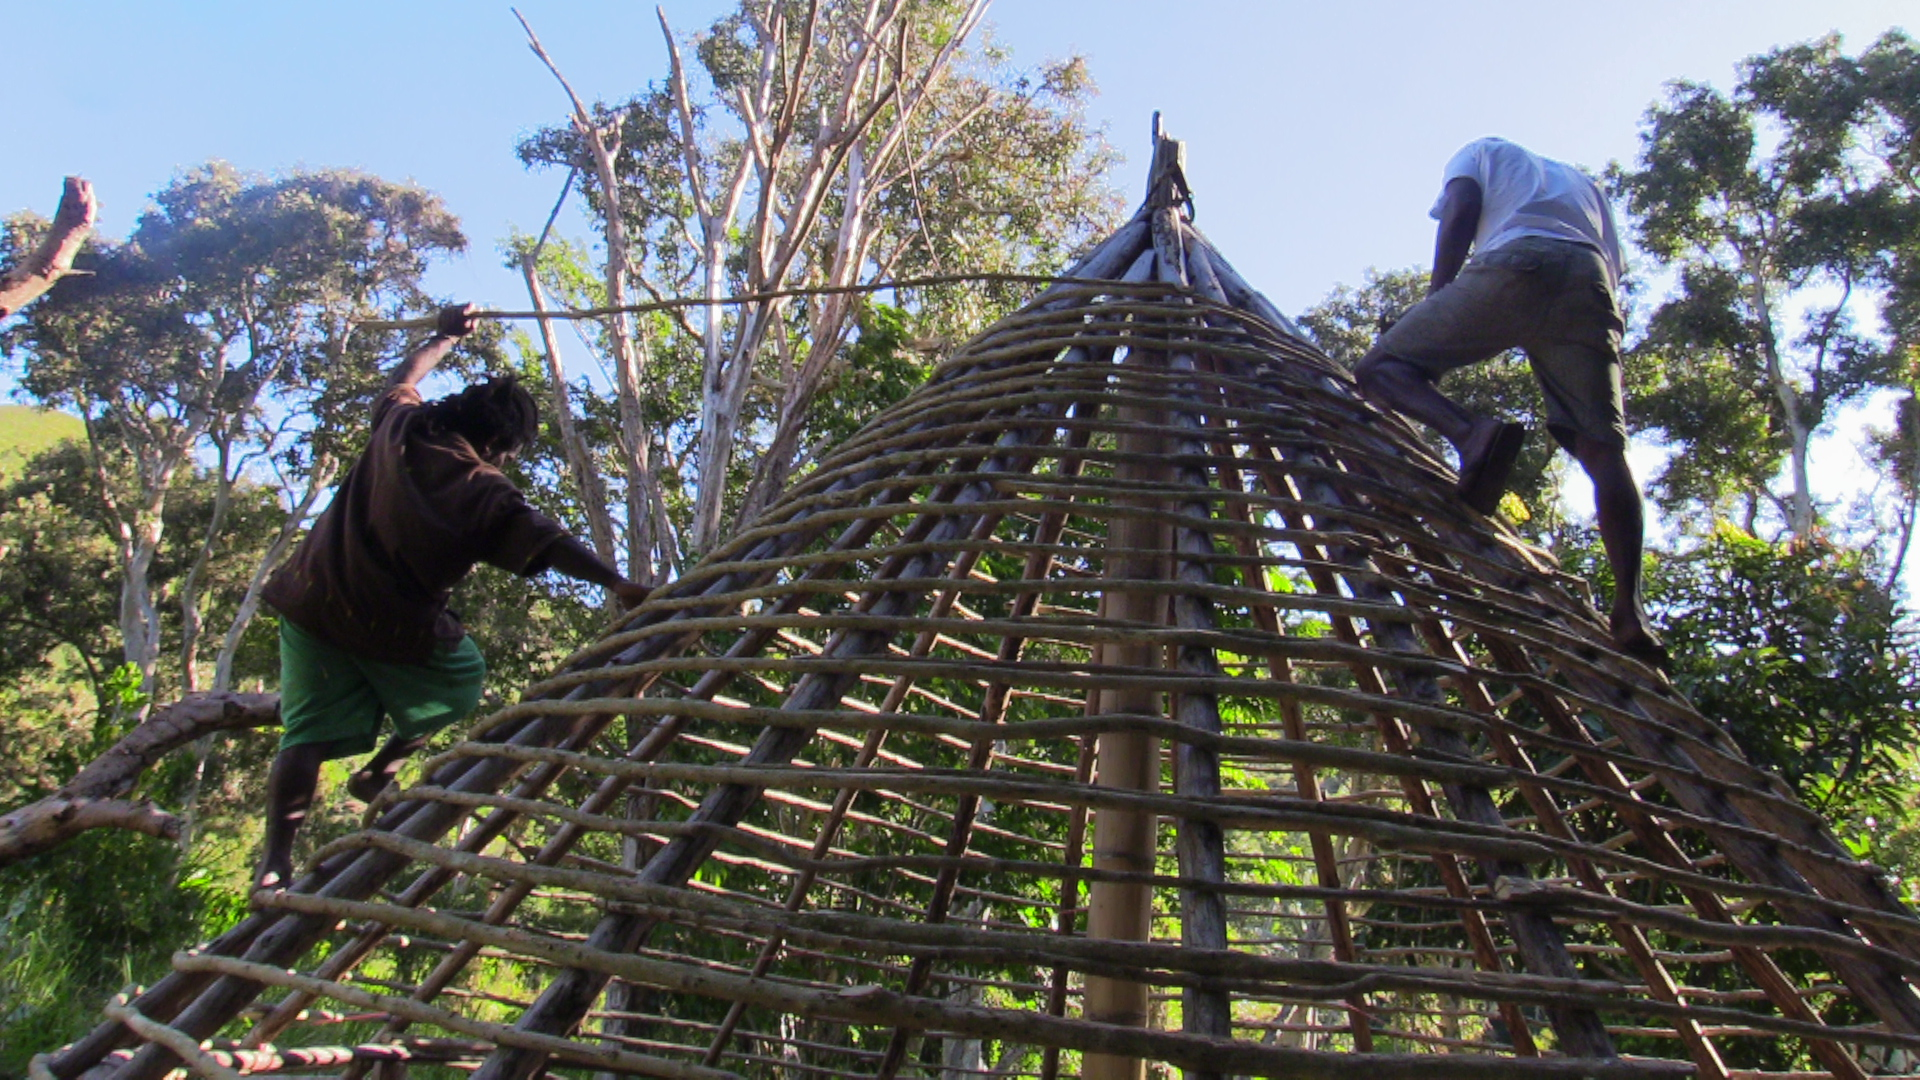
\includegraphics[width=\linewidth]{figures/house}
%\caption{Building a house requires many parts.}
%\end{figure}
